\documentclass[titlepage]{jsarticle}
\usepackage[dvipdfmx]{graphicx}
\usepackage{url}
\usepackage{amsmath}
\usepackage{comment}
\usepackage[version=3]{mhchem}
\usepackage{otf}
\title{14.フォトニクス実験}
\author{学生番号03180523 渡辺耕坪}
\date{\today}
\begin{document}
\maketitle

\begin{comment}
\begin{figure}[htbp]
 \begin{minipage}{0.5\hsize}
  \begin{center}
   \includegraphics[width=80mm]{}
  \end{center}
  \caption{}
  \label{}
 \end{minipage}
 \begin{minipage}{0.5\hsize}
  \begin{center}
   \includegraphics[width=80mm]{}
  \end{center}
  \caption{}
  \label{}
 \end{minipage}
\end{figure}
\end{comment}

\begin{comment}
\begin{figure}[htbp]
 \begin{minipage}{0.5\hsize}
  \begin{center}
   \includegraphics[width=80mm]{}
  \end{center}
  \caption{}
  \label{} \end{minipage}
\end{figure}
\end{comment}
\section{Abstract}
フォトニクス実験では半導体レーザー、超短パルスファイバレーザ、空間光学の三つに関する実験を行った。このうち超短パルスファイバレーザに関しては実験の原理、実験結果、詳細な考察を提出し、空間光学、半導体レーザーに関しては簡略な実験結果といくつかの考察のみをレポートとして提出する。
\section{Introduction}
\subsection{超短パルスファイバレーザ}
光の広い周波数帯域を利用して、時間領域で極めて狭い間のみに光パワーが集中しているパルスを発生させることができる。今回の実験ではファイバレーザを用いてパルスを発生させる。また、パルスを用いて超短パルスの時間幅を、応答時間が長いフォトディテクタによって観測する自己相関法による解析を行い、スペクトラムアナライザによって得られた結果と比較する。
\subsection{実験の原理}
\subsubsection{超短パルスファイバレーザ}

\subsection{実験装置}
オシロスコープ
スペクトラムアナライザ
半導体レーザドライバ
温度コントローラ
波形発生装置
直流電流
パソコン
\subsection{実験方法}
\subsubsection{半導体レーザー}



\subsubsection{空間光学}



\subsubsection{超短パルスファイバレーザ}
1.ファイバレーザのモード同期\\
    ファイバレーザ発生システム内の個々の機器の電源を投入し、レーザ注入電流を700mAに設定する。オシロスコープで波形を見ながらシステム内の三枚の波長版を回転させ、パルスが発生するように調整する。\\
2.単一パルスを発生させる\\
    発生させたパルスはオシロスコープの表示では単一のパルスに見えるが、スペクトラムアナライザで周波数成分を見ると単一のパルスではないことが分かる。そこで、で注入電流を下げていき、スペクトル分布がどのように変化していくかを記録す
    る。\\
3.自己相関波形の解析\\
    図\ref{fig;palse_laser}の実験系を用いて単一パルスを二つに分け、経路によって時間差がついた二つの波形の重ね合わせを、二つのフォトディテクターによって観測する実験である。本来は発生させた単一パルスを用いてこの実験を行う予定だったが、実験系の不調により、あらかじめ以上の実験系を用いて行われた実験データを用いて以下の解析を行う。\\
    1.PD\\
        \ce{InGaAs}を材料とするフォトディテクターで、受光した光波の振幅の2乗に比例した電流を発生させる。\\
    2.TPA-PD\\
        \ce{GaAsP}を材料とするフォトディテクターで、受講した硬派の振幅の4乗に比例した電流を発生させる。\\
    それぞれ観測した電流を用いて離散フーリエ変換によって光スペクトルを得ることができる。これによって得られた光スペクトルを別途、スペクトラムアナライザによって得た結果と比較する。\\



\section{Results}
\subsection{半導体レーザー}

\subsection{空間光学}

\subsection{超短パルスファイバレーザー}
\begin{figure}[htbp]
 \begin{minipage}{0.5\hsize}
  \begin{center}
   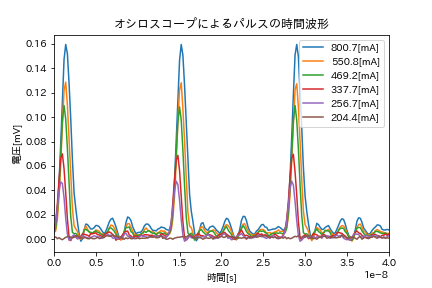
\includegraphics[width=80mm]{palse_osiro.png}
  \end{center}
  \caption{パルスをオシロスコープによって観測した結果。注入電流が大きい場合はパルスの大きさが大きいがパルス幅が広くなっている。また、注入電流が小さすぎるとノイズのみが出力されている。}
  \label{} \end{minipage}
\end{figure}
\begin{figure}[htbp]
 \begin{minipage}{0.5\hsize}
  \begin{center}
   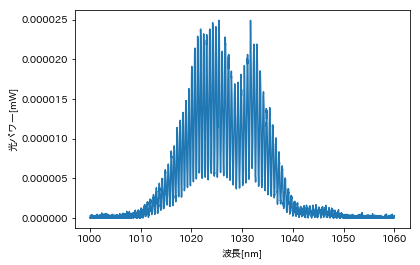
\includegraphics[width=80mm]{800_7[mA].png}
  \end{center}
  \caption{800.7[mA]の注入電流によるスペクトル。}
  \label{fig:800_7}
 \end{minipage}
 \begin{minipage}{0.5\hsize}
  \begin{center}
   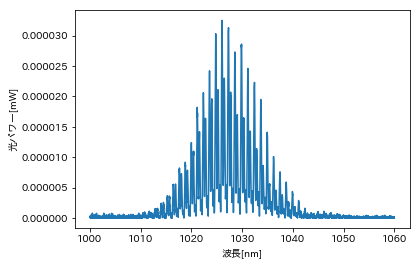
\includegraphics[width=80mm]{550_8[mA].png}
  \end{center}
  \caption{550.8[mA]の注入電流によるスペクトル。}
  \label{fig:550_8}
 \end{minipage}
\end{figure}
\begin{figure}[htbp]
 \begin{minipage}{0.5\hsize}
  \begin{center}
   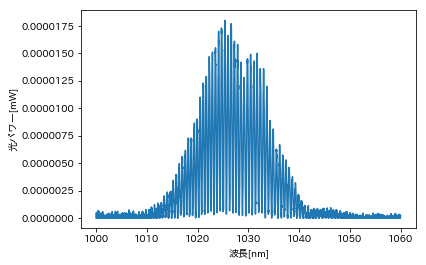
\includegraphics[width=80mm]{469_2[mA].png}
  \end{center}
  \caption{800.7[mA]の注入電流によるスペクトル。}
  \label{fig:469_2}
 \end{minipage}
 \begin{minipage}{0.5\hsize}
  \begin{center}
   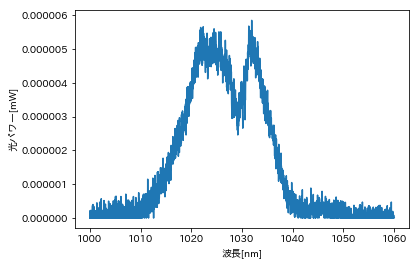
\includegraphics[width=80mm]{337_7[mA].png}
  \end{center}
  \caption{337.7[mA]の注入電流によるスペクトル。スペクトルの振動が消失している。}
  \label{fig:337_7}
 \end{minipage}
\end{figure}
\begin{figure}[htbp]
 \begin{minipage}{0.5\hsize}
  \begin{center}
   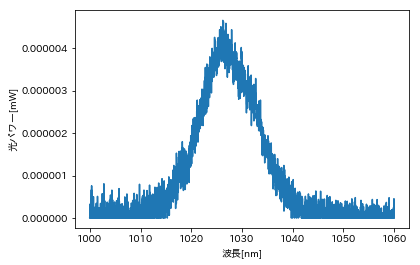
\includegraphics[width=80mm]{256_7[mA].png}
  \end{center}
  \caption{256.7[mA]の注入電流によるスペクトル。ガウシアンに近いスペクトル分布が得られた。}
  \label{fig:256_7}
 \end{minipage}
 \begin{minipage}{0.5\hsize}
  \begin{center}
   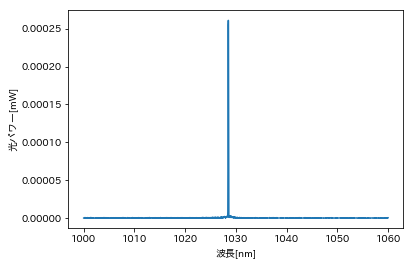
\includegraphics[width=80mm]{204_4[mA].png}
  \end{center}
  \caption{204.4[mA]の注入電流によるスペクトル。ほとんど周波数に依存する成分を得られなかったので$\delta$関数的なスペクトル分布になっている。}
  \label{fig:204_4}
 \end{minipage}
\end{figure}
\clearpage
\section{Discussion}
\subsection{半導体レーザー}
五つある発表課題のうち発表課題5について考察を行う。\\
\subsection{超短パルスレーザー}
検討課題1~4と7について考察を行う。
1.
\begin{equation}
    S(t)=\frac{1}{2}[\varepsilon(t)e^{j\omega_0 t}+c.c](c.cは直前項の複素共役を表す)
    \label{eq1_1}
\end{equation}
\begin{equation}
    S(\omega)=\frac{1}{2}[E(\omega-\omega_0)+E^{*}(-\omega-\omega_0)]
    \label{eq1_2}
\end{equation}
式\ref{eq1_1}をフーリエ変換し$S(\omega)とE(\omega)$が式\ref{eq1_2}の関係となっていることを示す。\\
2.レーザーからダブルパルスが出力されているときスペクトルが振動する理由。また、振動周期から推定されるダブルパルスの時間幅について。\\
3.レーザの平均パワーが10[W]程度であると仮定し、繰り返し周波数
とパルス幅を用いてピークパワーを推定する。\\
4.計測された光パルスの時間幅は光の何周期分か推定する。また、スペクトル幅と中心周波数の比と、両者の関係について。\\
7.ガウシアンパルスのスペクトル位相が$\Phi(\omega)=-\frac{1}{2}\Phi_2\omega^2$であるときの時間波形の計算。\\


\section{Summary}


\begin{thebibliography}{9}
  \bibitem{}
  \bibitem{}
\end{thebibliography}
\end{document}

